\section{Introduction}\label{intro}
Universe

Accuracy

No 

Inverse Problems

\subsection{Radio Interferometry}
\begin{figure}[h]
	\centering
	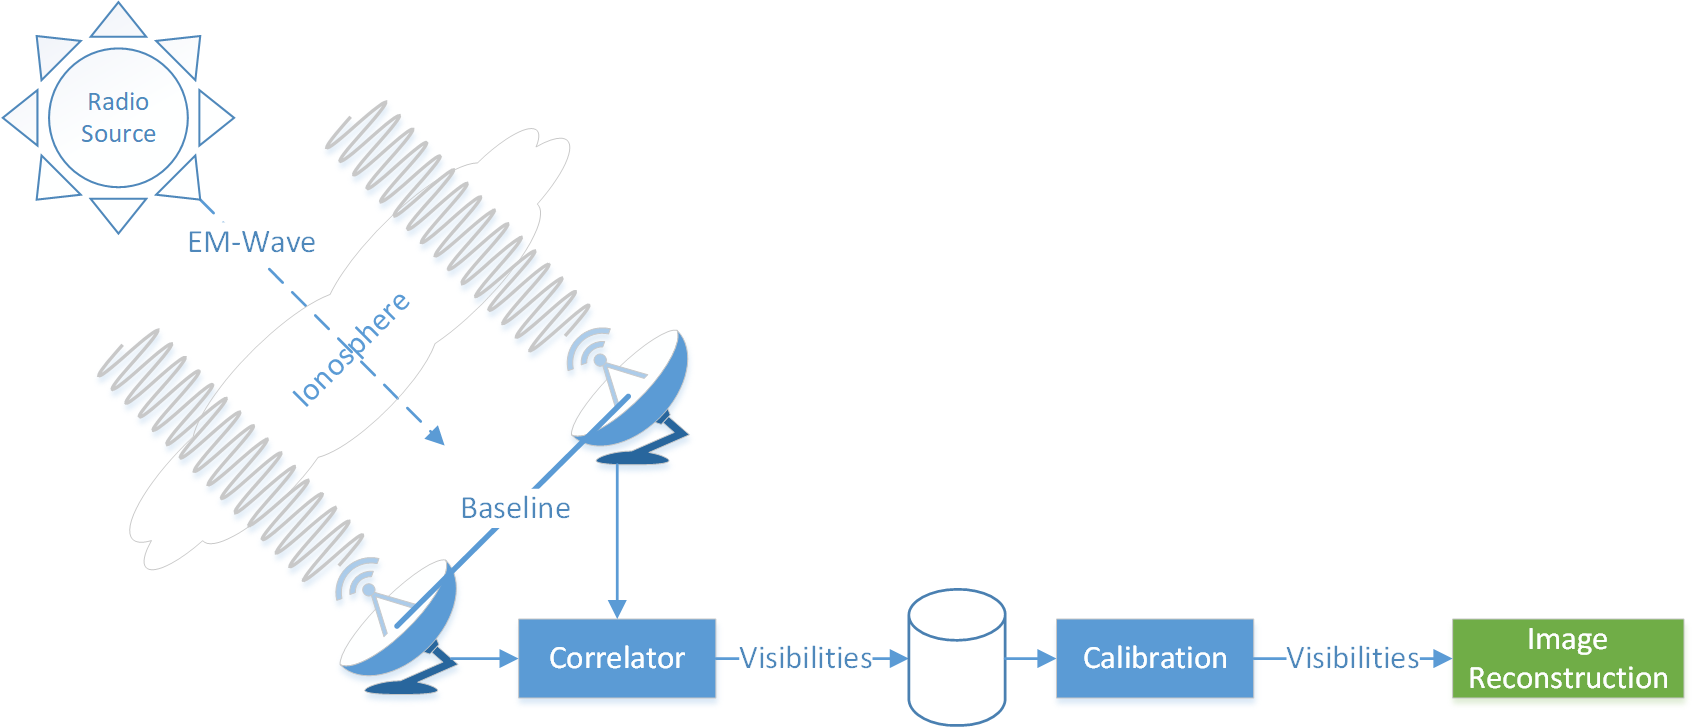
\includegraphics[width=0.80\linewidth]{./chapters/01.intro/system.png}
	\caption{Interferometer System}
	\label{intro:system}
\end{figure}

\subsection{Inverse Problem}




\begin{equation}\label{intro:ftsphere}
V(u, v, w) = \int\int \frac{I(x, y)}{\sqrt{1 - x^2 - y ^2}} e^{2 \pi i [ux+vy+ w(\sqrt{1 - x^2 - y ^2} - 1)]} \: dx \: dy
\end{equation}



\subsection{Image Reconstruction}

\subsection{State of the art Deconvolution algorithms}

CLEAN

Compressed Sensing

What is a deconvolution algorithm

\pagebreak
\section{Distributed Image Reconstruction for Radio Interferometers}
In Astronomy, instruments with higher angular resolution allows us to measure ever smaller structures in the sky. For Radio frequencies, the angular resolution is bound to the antenna dish diameter, which puts practical and financial limitations on the highest possible angular resolution. Radio Interferometers get around this limitation by using several smaller antennas instead. Together, they act as a single large antenna with higher angular resolution at lower financial costs compared to single dish instruments.

Each antenna pair of an Interferometer measures a single Fourier component of the observed image. We can retrieve the image by calculating the Fourier Transform of the measurements. However, since the Interferometer only measures an incomplete set of Fourier components, the resulting image is "dirty", convolved with a Point Spread Function ($PSF$). Calculating the Fourier Transform is not enough. To reconstruct the from an Interferometer image, an algorithm has to find the observed image with only the dirty image and the $PSF$ as input. It has to perform a deconvolution. The difficulty lies in the fact that there are potentially many valid deconvolutions for a single measurement, and the algorithm has to decide for the most likely one. How similar the truly observed image and the reconstructed images are depends largely on the deconvolution algorithm.

State-of-the-art image reconstructions use the Major Cycle architecture (shown in figure \ref{hypo:major3}), which contains three operations: Gridding, FFT and Deconvolution.

\begin{figure}[h]
	\centering
	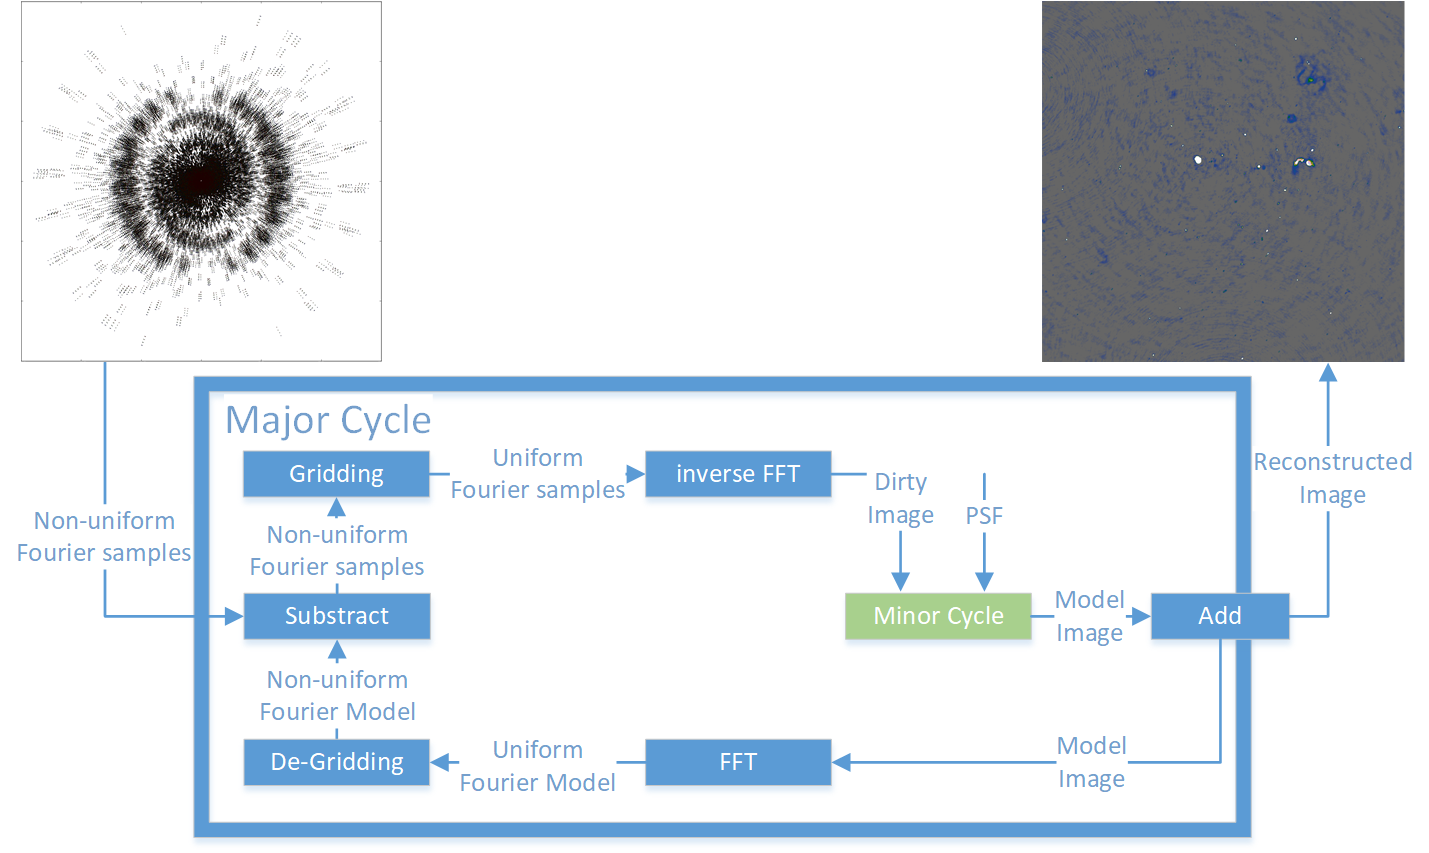
\includegraphics[width=0.80\linewidth]{./chapters/02.hypo/Major-Minor3.png}
	\caption{The Major Cycle Architecture of image reconstruction algorithms}
	\label{hypo:major3}
\end{figure}

The first operation in the Major Cycle, Gridding, takes the non-uniformly sampled Fourier measurements from the Interferometer and interpolates them on a uniformly spaced grid. The uniform grid lets us use FFT to calculate the inverse Fourier Transform and we arrive at the dirty image. A deconvolution algorithm takes the dirty image plus the $PSF$ as input, producing the deconvolved "model image", and the residual image as output. At this point, the reverse operations get applied to the residual image. First the FFT and then De-gridding, arriving at the non-uniform Residuals. The next Major Cycle begins with the non-uniform Residuals as input. The cycles are necessary, because the Gridding and Deconvolution operations are only approximations. Over several cycles, we reduce the errors introduced by the approximate Gridding and Deconvolution. The final, reconstructed image is the addition of all the model images of each Major Cycle. 

\subsection{Distributed computing for Large Scale Reconstructions}
New Interferometer produce an ever increasing number of measurements, creating ever larger reconstruction problems. A single image can contain several terabytes of Fourier measurements. Handling reconstruction problems of this size forces us to use distributed computing. However, state-of-the-art Gridding and Deconvolution algorithms only allow for limited distribution. How to scale the Gridding and Deconvolution algorithms to large problem sizes is still an open question.

Recent developments make a distributed Gridder and a distributed Deconvolution algorithm possible. Veeneboer et al\cite{veenboer2017image} found an input partitioning scheme, which allowed them to perform the Gridding on the GPU. The same partitioning scheme can potentially be used to distribute the Gridding onto multiple machines. For Deconvolution, there exist parallel implementations for certain algorithms\cite{dabbech2015moresane}. These can be used as a basis for distributed implementations.

In this project, we want to make the first steps towards distributed image reconstruction, creating a distributed Gridding and distributed Deconvolution algorithms and comparing the reconstruction quality to state-of-the-art algorithms.

\subsection{First steps towards distributed Image Reconstruction}
In this project, we make the first steps towards a distributed Major Cycle architecture (shown in figure \ref{hypo:major3}) implemented C\#. The whole pipeline will be a proof-of-concept implementation. We ignore the fact that the Radio Interferometer measurements are polarized, which allows us to simplify the implementation of the Gridder and Deconvolution algorithm. The first image reconstruction pipeline will be created in three steps.

We start with a distributed Deconvolution algorithm based on the previous project 8. In this step, we can use the Veeneboer et al's Gridder as-is, without modification and have a working image reconstruction pipeline.

In the second step we create a distributed Gridder based on Veeneboer et al's input partitioning scheme. We can verify the correctness of our modifications by comparing its output to the original implementation. 

The third step is to create a more sophisticated Deconvolution algorithm based on the shortcomings of the first implementation. We use simulated and real-world Radio Interferometer observations and compare the reconstruction quality of our approach to state-of-the-art algorithms. We identify the bottlenecks of the current pipeline and explore further steps.

Possible Further steps:
\begin{itemize}
	\item Distributed FFT
	\item Replacing the Major Cycle Architecture
	\item GPU Deconvolution implementation.
\end{itemize}





